\newpage
\section{Practical 1 - Testing methodologies}
\label{sec:Prac1}

\subsection{Introduction}
This practical will have you work with concepts of golden measure, execution time, critical path and speed up, using correlation of pink and white noise as a framework for testing.

\subsubsection{Correlation}
Correlation is a useful statistical function for comparing two datasets to judge how similar or different they are. The correlation function returns a correlation coefficient, r, between -1 and 1. A value of 1 for r implies perfect positive correlation, i.e. the two datasets are the same. Correlation of 0 implies there is no correlation (the two datasets behave totally differently). A correlation of -1 indicates a total opposite - for example if you compare vectors x to - x you get a correlation of -1. Generally if $|r| >= 0.8$ there is strong correlation, between 0.5 and 0.8 moderate weak, less that 0.5 is weak (towards no) correlation.

Pearson's correlation (which you can read more about on \href{https://en.wikipedia.org/wiki/Pearson_correlation_coefficient}{Wikipedia}) is implemented as follows:
\begin{equation}
\label{eqn:Pearson}
  r =
  \frac{ \sum_{i=1}^{n}(x_i-\bar{x})(y_i-\bar{y}) }{%
        \sqrt{\sum_{i=1}^{n}(x_i-\bar{x})^2}\sqrt{\sum_{i=1}^{n}(y_i-\bar{y})^2}}
\end{equation}

\subsubsection{Speed Up}
\begin{equation}
Speedup = \frac{T_{p1}}{T_{p2}}
\end{equation}
Where:\\
$T_{p1}$ = Run-time of original / non-optimal program\\
$T_{p2}$ = Run-time of optimised program

For obtaining a repeatable timing value, run each version (i.e. initial version and optimised version) of your programs more than once and discard the first measured time. You can, if you want to be complete, indicate what the initial speed up was and then the average speed up.

\subsubsection{Pink Noise}
Watch to \href{https://www.youtube.com/watch?v=NO2xgLAfQac}{this video}.

Pink noise is a random signal, filtered to have equal energy per octave. In order to keep the energy constant over octaves, the spectral density needs to decrease as the frequency (f) increases. This explains why pink noise is sometimes referred as "1/f noise." In terms of decibels, this decrease corresponds to 3 dB per octave on the magnitude spectrum. The name of the color comes from visible light that turns pink when a similar spectral distribution is applied. \cite{pinknoise}

\subsection{Requirements}
For this practical, you will need a machine that runs the programming language Julia.
\begin{itemize}
    \item A system that runs Julia
    \item The latest Prac files off \href{https://github.com/kcranky/EEE4120F_Pracs}{Github}
    \item sudo apt-get install qt5-default
\end{itemize}

\subsection{Tasks}
\subsubsection{Generate White Noise}
The code below is adapted from \href{https://stackoverflow.com/a/53405121/1676144}{this Stackoverflow answer}.
Considering white noise is Gaussian distributed, we can use the rand() function to generate random samples. 
The pink noise sample we're working with is 10 seconds long, and is sampled at 44100Hz. That means we need to create 10*44100 = 441000 +1 = 441001 random numbers in the range [-1, 1]. The pink noise source uses 16 bit numbers, so we need to use 16 bit numbers for our whitenoise generator, too.

\begin{enumerate}
    \item Start by opening a terminal where you downloaded the Prac 1 files, and running \verb|$ julia packages.jl|. This will ensure that all the packages required for this practical are installed.
    \item Create a new file called \verb|whitenoisegenerator.jl|
    \item In it, enter the following code. Don't do so blindy, try and understand what the code is doing.
    \begin{lstlisting}[gobble=8]
        # Import the required libraries
        using WAV
        using Random
        # import the Plots library and set the plotting backend
        using Plots
        pyplot()

        # Tell julia we want this function accessible outside this package
        export genwhitenoise 
        
        # write the function to generate white noise
        function genwhitenoise()
	        white = (rand(10*44100+1) .* 2 .- 1)
	        wavwrite(white, "whitenoise.wav", Fs=44100) # save to file
	
	        # create a histogram to check the samples and distribution
        	p = histogram(white[1:1000])
	        savefig(p, "whitenoise_hist.png")
	
        end 
        # call the function to run it
        genwhitenoise()
    \end{lstlisting}
    This function allows us to generate white noise for a given number of samples at a sampling rate of 44100Hz for 10 seconds. We need to use element-wise multiplication and subtraction on the rand() function to get values in [-1, 1].
    \item Once you've confirmed  that the histogram looks as expected, you remove the following lines from your code:
    \begin{lstlisting}[gobble=8]
        # import the Plots library and set the plotting backend
        using Plots
        pyplot()
        ...
        
        # create a histogram to check the samples and distribution
        p = histogram(white[1:1000])
        savefig(p, "whitenoise_hist.png")
	\end{lstlisting}
\end{enumerate}

\subsubsection{Correlate Pink and White Noise}
Start by implementing your correlation function in a new file, called \verb|my_corr.jl|. In it, implement the Pearson correlation function, as given in Equation \ref{eqn:Pearson} above.

Compare the results of your correlation function to the results of the inbuilt correlation function.

To read in the pink noise, use the \verb|wavread| function from the \verb|WAV| package:\\
\verb|data_pink, Fs_pink, nbits_pink, opt_pink = wavread("pinknoise.wav")|
You can read more about the WAV package \href{https://github.com/dancasimiro/WAV.jl}{here}. 

Before you being, get a histogram plot of the first few thousand pink noise samples.

\subsubsection{Measuring Execution Time}
\textbf{TODO}
@time function

\subsubsection{Compare Speed Up using multiple threads}
Julia uses threads by default. To see how many threads Julia is currently making use of, open a terminal, run \verb|$julia| and in the julia terminal, run \verb|Threads.nthreads()|.

\begin{figure}[H]
\centering
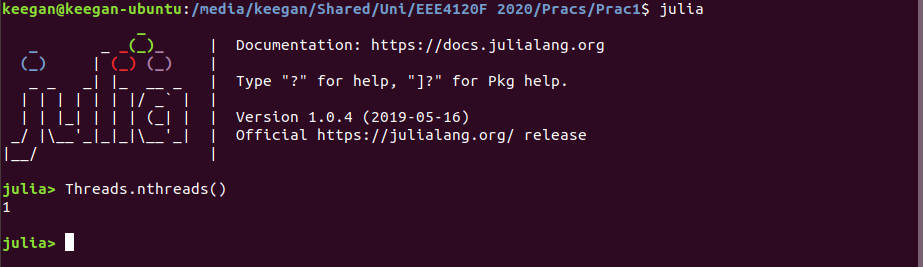
\includegraphics[width=0.6\columnwidth]{Figures/julia-singlethread}
\caption{Julia using a single thread}
\label{fig:julia-singlethread}
\end{figure}

Exit the Julia terminal by pressing \verb|ctrl+D|.

We can change the number of threads Julia uses by running \verb|$ export JULIA_NUM_THREADS=n| in a terminal, where n is the number of threads we want to use. For example, if we do n=4, and run Julia to test the number of threads, we get:

\begin{figure}[H]
\centering
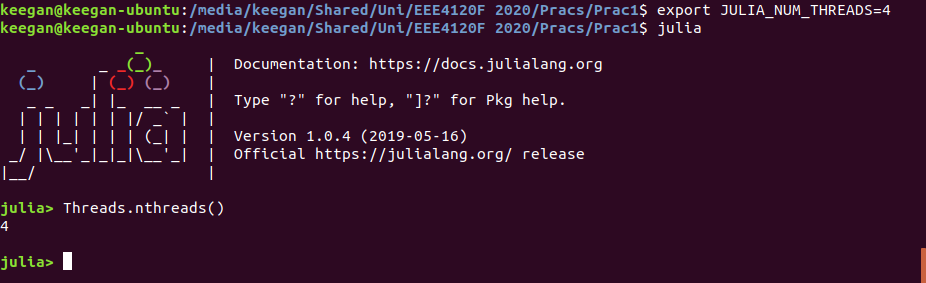
\includegraphics[width=0.6\columnwidth]{Figures/julia-manythreads}
\caption{Julia using many threads}
\label{fig:julia-manythreads}
\end{figure}

For different sample sizes (different durations of the signal), test the speed of your correlation function against the speed of the inbuilt correlation function.

\subsection{Submission}
Hand in a short report (aim for two pages: the page limit for this assignment is 3) briefly describing your solutions for the tasks above. The format required is the IEEE conference format. Format your report as if it is an article (i.e. don’t follow the same chronology as the prac-sheet – format it as “Introduction – Method – Results and Discussion – Conclusion”). In the ``Method" section, theorise about what you expect and how you plan on testing said theory. In the ``Results" section, confirm that you obtained what you expected (or explain why you obtained something unexpected). Hint: You are trying to answer two questions: 1) ``Is my mycorr function better suited to run correlation tests, in comparison to the built-in equivalent?" and 2) ``How similar is pink noise to white noise?"

\subsection{Marking}
Report	
    Intro (2)
	Latex/Format (1)
	Headings etc (1)
	Captions (1)
	
createwhiten	
    Code intro concepts (4)
	Neatness (3)
	Structure (3)
	
Sz. v t	
    Table (2)
	Graph (1)
	Explanation (2)
	
Shifted signals	
    Screenshots (2)
	Code (2)
	Correlation (2)
	Explanation (3)
	Expected vs Results (1)